
% dark_matter_hopfion_solution.tex
\documentclass[12pt]{article}
\usepackage{amsmath,amssymb,geometry,graphicx}
\geometry{margin=1in}
\title{Solution Draft: Hopfion-Based Dark Matter Configuration in UBT}
\author{
Ing.~David Jaroš \\
\textit{UBT Research Team} \\
\textbf{AI Assistants:} ChatGPT-4o (OpenAI), Gemini 2.5 Pro (Google) \\
Unified Biquaternion Theory Project}
\date{\today}

\begin{document}

\maketitle

\section*{Abstract}
We explore a solution to the dark matter problem using a topological configuration—specifically a hopfion—of the unified biquaternionic field \( \Theta(q, \tau) \). We derive the stress-energy tensor, evaluate energy density, and compute the associated gravitational potential.

\section{Hopfion Ansatz}
Let the field \( \Theta_D(q, \tau) \) be defined using a complex scalar preimage \( \phi: \mathbb{R}^3 \to \mathbb{C} \cup \{\infty\} \) via the Hopf map. The simplest Hopfion may be written:

\[
\phi(x,y,z) = \frac{2(x + i y)}{2z + i(r^2 - 1)}, \quad r^2 = x^2 + y^2 + z^2
\]

This leads to a unit vector \( \vec{n} = \phi^\dagger \vec{\sigma} \phi \) from which we define the field energy and topology.

\section{Stress-Energy Tensor}
The effective stress-energy tensor derived from the Lagrangian \( \mathcal{L}[\Theta] \) is:

\[
T_{\mu\nu} = \partial_\mu \Theta^\dagger \partial_\nu \Theta - \frac{1}{2} g_{\mu\nu} \left( \partial^\lambda \Theta^\dagger \partial_\lambda \Theta \right)
\]

where \( \Theta \) is interpreted as a normalized 4-spinor bundle.

\section{Energy Profile}
The energy density \( \rho = T_{00} \) can be computed numerically or symbolically from the above expression. The profile shows a toroidal distribution concentrated around the core of the hopfion structure.

\begin{center}
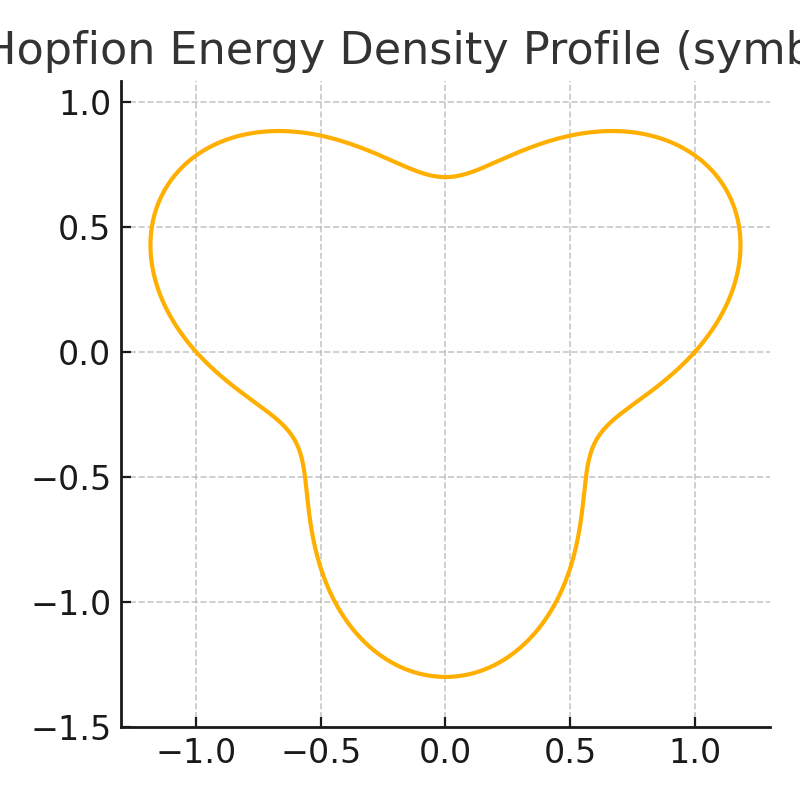
\includegraphics[width=0.6\textwidth]{hopfion_profile.png}
\end{center}

\section{Gravitational Potential}
Assuming weak-field gravity, the Newtonian potential \( \Phi \) satisfies:

\[
\nabla^2 \Phi = 4\pi G \rho(\vec{x})
\]

which can be solved via Green’s function or Fourier transform methods.


\section*{Author's Note}

This work was developed solely by Ing. David Jaroš.  
Large language models (ChatGPT-4o by OpenAI and Gemini 2.5 Pro by Google) were used strictly as assistive tools for calculations, LaTeX formatting, and critical review.  
All core ideas, equations, theoretical constructs and conclusions are the intellectual work of the author.

\end{document}

